\documentclass[a4paper]{article}

\usepackage[english]{babel}
\usepackage[utf8]{inputenc}
\usepackage{amsmath}
\usepackage{amssymb}
\usepackage[style=numeric, backend=bibtex]{biblatex}
\usepackage{graphicx}
\usepackage[colorinlistoftodos]{todonotes}
\usepackage{pgfplots}
\usepackage{pgfplotstable}

\usepackage{float}
\floatstyle{boxed}
\restylefloat{figure}

\addbibresource{main.bib}

\title{Euler vs. Hamilton --- Investigating Claims of Quaternion Superiority for Rotation Parameterization of Interactive 3D Camera Control Problems}
\author{}
\date{}

\begin{document}
\maketitle

\section{Introduction}

Rotation --- or rather the \emph{representation} of rotation --- in three-dimensional affine space is surprisingly difficult.
There are many different ways to represent these rotations, e.g. Euler-angle, axis-angle, rotation matrices, or unit quaternion parameterizations.
Of these examples, the unit quaternion parameterization is often said to be superior.
Quaternions solve the gimbal lock problems that Euler-angle systems experience, and are said to be more numerically stable.
It has also been claimed that Quaternions are a more efficient method of calculating rotations.
We have no reason to doubt these claims, in fact they seem sensible to us and we present empirical evidence of their veracity.
However, we question the conclusion that all animation systems should use quaternions as a parameterization of their rotations.
In this paper we will specifically look at the special case of an interactive three dimensional camera with three degrees of freedom (pitch, roll and yaw) in order to see whether the claims that quaternions are superior can be empirically supported.
These claims are that Quaternions do not suffer from gimbal lock; are more numerically stable than other approaches; and more performant.
To the best of the authors' knowledge, there are no research papers that publish empirically derived figures supporting these claims.
It is important to have access to such figures, however, since what is true in theory may not hold up in practise once implemented on a real computer system ---
especially due to factors such as the numerical instability that is introduced by the inaccurate floating point mathematics as implemented for computers, or the fact that graphics cards and their drivers may have hidden performance cliffs and undocumented behaviour.
We have also been unable to find any discussion in the literature about which parameterization to use for floating cameras with three degrees of freedom.
The contribution of this paper is then a conclusion as to this best possible parameterization and the provision of empirical figures to back up various claims.

\section{Parameterizations}

Several parameterizations of rotations in three dimensions have already been proposed.
We recapitulate some of them here, for the uninitaited reader.

\subsection{Euler-Angle}

The Euler-angle system is a parameterization based on three separate angles: roll, pitch and yaw --- these are the rotation amounts around three separate axes: the X, Y, and Z axes, respectively \parencite[11]{diebel06}.
The problem with this system is one of gimball lock.
Briefly stated, a rotation of one of the axes can bring it into the plane of one of the other axes.
At this stage, a rotation about any one of these two axes is equivalent to a rotation about the other, we have therefore lost a degree of freedom \parencite[4]{pletinckx89}.

\subsection{Axis-Angle}

The axis-angle representation collapses all rotations to a rotation with a certain magnitude about a single axis.
The magnitude of this rotation becomes the length of a vector with a direction that corresponds to this axis \parencite[18]{diebel06}.

\subsection{Rotation Matrices}

Rotation matrices represent rotations as the components of a $3 \times 3$ matrix of real vlaues.
Rotation matrices are convenient because they work well with the well-established method of using matrices to represent affine transformations in computer graphics applications.
Rotation matrices have to be kept ortho-normal, if they deviate from this property then they will alter the length of vectors, leading to distortions in the shape of the objects being rotated \parencite[4--5]{diebel06}.

\section{Experimental Setup}

Our experiment consists of an implementation of both competing methods of interactive camera control.
The first implementation stores the current camera's position and orientation as a view matrix.
This view matrix is then multiplied by a rotation or translation matrix that indicates the amount to rotate or move by whenever the camera's position is altered.
The second implementation stores the current camera's position and orientation as a quaternion.
The quaternion is then multiplied by another quaternion that indicates the adjustment in the camera's position or orientation whenever a movement key is pressed or the mouse is moved.
We implement these camera classes as C++ templates and parameterize them as both doubles and floats.
Each implementation is also accompanied by a version that ortho-normalizes the rotation sub-matrix before it is sent to the shaders to be used as a view matrix.

\begin{figure}
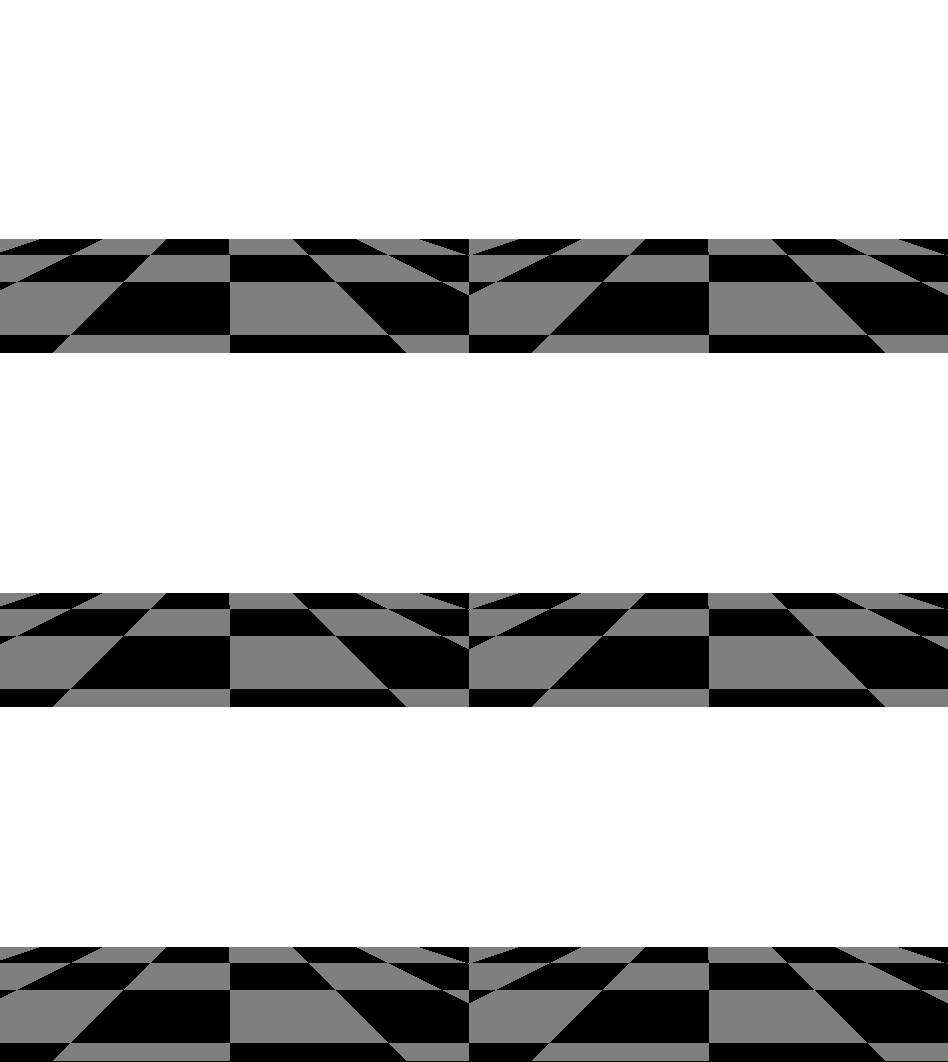
\includegraphics[width=12cm]{user_interface.png}
\caption{The user interface for the test platform.}
\end{figure}

The user is now presented with a simple scene that contains some basic geometry to allow the user to orient him / herself.
By moving the mouse, the user can rotate the camera about its X or Y axes.
Keyboard controls allow the user to move the camera forward, back and to the left and right.
The keyboard also allows the user to ``roll'' the camera around the Z axis.

With each alteration of the camera's position or orientation we obtain the resulting view matrix for each algorithm's single precision and double precision versions.
For each element of the view matrix, we subtract the single precision value from the double precision value.
We assume that the latter will be more accurate than the former.
Therefore, this subtraction indicates the amount of error in the single precision value.
We sum the result of each of these subtractions to obtain an overall error value for that algorithm.

Next, the algorithms are compared against one another for each mouse / keyboard movement.
If an algorithm has an error value that is less than that of its competitor, it is awarded a win.
At the end of the test run, the algorithm with the most wins is deemed the most numerically stable.

Thirty tests of approximately one minute each were run, recording the victorious algorithm after each test has terminated.

\section{Results} 

An interesting result is that the quaternion algorithms are actually faster than the rotation matrix versions.
This is in line with the passing comment made by Taylor \parencite[435]{taylor79}.

There is good mathematical basis for this as well.
Consider a case where a view matrix representation has to be updated with a rotation around two axes, for example the X and Y axes.
(We ommit the Z axis from this consideration, because it is implemented in exactly the same way as the X and Y axes, and therefore doesn't affect a comparison between methods if it is left out.)
The view matrix itself is a four dimensional matrix in homogenous coordinate space, and so is the rotation matrix for the X and Y axes.
The current view matrix is given by:

\vspace{0.5em}
$V = \left[ \begin{array}{cccc}
    V_{11} & V_{12} & V_{13} & V_{14} \\
    V_{21} & V_{22} & V_{23} & V_{24} \\
    V_{31} & V_{32} & V_{33} & V_{34} \\
    V_{41} & V_{42} & V_{43} & V_{44} \\
\end{array} \right]$

Then the X and Y update matrices are given by:

\vspace{0.5em}
$X = \left[ \begin{array}{cccc}
    X_{11} & X_{12} & X_{13} & X_{14} \\
    X_{21} & X_{22} & X_{23} & X_{24} \\
    X_{31} & X_{32} & X_{33} & X_{34} \\
    X_{41} & X_{42} & X_{43} & X_{44} \\
\end{array} \right]$, and
$Y = \left[ \begin{array}{cccc}
    Y_{11} & Y_{12} & Y_{13} & Y_{14} \\
    Y_{21} & Y_{22} & Y_{23} & Y_{24} \\
    Y_{31} & Y_{32} & Y_{33} & Y_{34} \\
    Y_{41} & Y_{42} & Y_{43} & Y_{44} \\
\end{array} \right]$

The update step then involves an equation like $V\prime = VXY$ where $V\prime$ is the new view matrix.
This involves two $4 \times 4$ matrix-matrix multiplications, which can be decomposed into two sets of dot products between the columns and rows of each matrix.
Since each matrix is $4 \times 4$, this is approximately 32 dot products in total.
Each dot product contains 3 summation operations and 4 multiplies, which leads to a total of 96 summations and 128 multiplies for the matrix-matrix multiplication alone.
In addition, a further four transcendental function invocations each are required to calculate X and Y.
Finally, the Gram-Schmidt ortho-normalization process is applied, but since we applied this to the quaternio implementation here, it is not necessary to count its operations.

For the quaternion implementation, matters are different.
First, the quaternion rotations about the X and Y axes must be converted from an angle-axis.
This involves 2 transcendental function invocations as well as 5 multiplications for both the X and the Y quaternion, for a total of 4 transcendental function invocations and 10 multiplications \parencite{glm:quat:angleAxis}.
Next the quaternions must be multiplied.

Consider two quaternions: $q_1$ and $q_2$.
Now, each quaternion consists of one real part (which we can treat as a scalar) and an imaginary part (which we treat as a three-component vector).
Label these scalars and vectors as $s_1$, $s_2$, $v_1$, $v_2$, respectively.
If we rewrite $q_1$ as $\left[ \begin{array}{cc} s_1 & v_1 \end{array} \right]$ and $q_2$ as $\left[ \begin{array}{cc} s_2 & v_2 \end{array} \right]$ then quaternion multiplication is simply defined as $q_1 q_2 = \left[ \begin{array}{cc} s_1 s_2 - v_1 \cdot v_2 & s_1 v_2 + s_2 v_1 + v_1 \times v_2 \end{array} \right]$ \parencite{schoemake85}.

\section{Conclusion}

We have empirically verified various claims about unit quaternions and their use as rotation parameterizations.
They are somewhat faster than rotation matrices.
The difference is an order of magnitude, but the absolute values are already so low that it is likely that this difference will only matter in heavily resource-constrained environments.

\printbibliography

\end{document}
